\documentclass[a4paper]{article}
\usepackage{geometry}
\geometry{a4paper, portrait, margin=1.4in}
\usepackage[english]{babel}
\usepackage[utf8]{inputenc}
\usepackage{amsmath}
\usepackage{enumitem}
\usepackage{graphicx}
\usepackage[colorinlistoftodos]{todonotes}

\title{COL341: Machine Learning \\ \LARGE{Assignment 2 Report} \\ \Large{Neural Networks}}

\author{Utkarsh N. Singh, 2015ME10686}

\date{\today}

\begin{document}
\maketitle

\section*{Objective}
To develop and train a Neural Network to classify Devanagari Handwritten Characters. The dataset consists of 32x32 grayscale images and each image belongs to 46 different classes: 36 Devanagari characters and 10 Devanagari numerals. 

\section*{Part (a)}
For this part, a general neural network framework was to be implemented for the above problem from scratch using only numpy and pandas, which supports the following functionalities:
\begin{enumerate}
	\item Adding any number of hidden layers to the network with any number of hidden units
    \item Choosing the activation function across all the hidden units - ReLU, sigmoid or tanh
    \item Xavier initialization of weights for better convergence
    \item Setting batch size and initial learning rate
    \item Loss function is Mean Squared Error (MSE): $\frac{1}{N}\sum_{i=1}^{N} ||Y_i^2-\hat{Y_i}^2||^2$
\end{enumerate}
Above framework supports only fully connected architectures. Learning rate is decreased based on the average loss per epoch. This ensures that convergence is reached with minimal overshooting. The above design also ensures that the user can create any architecture they want for training over the Devanagari dataset.
\newline
\newline
\noindent Sigmoid was used as the activation function in the output layer.


\section*{Part (b)}
Given the training dataset of 78,200 examples, the objective was to obtain the best possible architecture for classifying the Devanagari Handwritten Characters into their respective classes and also to generalize well on unseen data.
\newline
\newline
Based on the training data size, an architecture with at most 2 hidden layers would be sufficient. Sigmoid was fixed as the activation function across all hidden units, and softmax activation function will be used in the output layer. 
\newline
\newline
Additionally, the loss function to be used was now the cross-entropy function:
\newline
\newline
\centerline{$L(Y_i, \hat{Y_i}) = -\frac{1}{N}\sum_{i=1}^{N}Y_ilog(\hat{Y_i})$}
\newline
\newline
With $Y_i$ being the one-hot encoding of the actual label, and $\hat{Y_i}$ the predicted probabilities for all the classes.
\newline
\newline
Using the method of holdout with 80:20 split of the training data, over 25 different architectures with varying batch sizes, learning rates and epochs were explored. Some of the promising models were: (bs - batch size, lr - initial learning rate)
\begin{enumerate}
	\item Layers = [500, 200], bs = 100, epochs = 100, lr = 1.4. Validation Accuracy = 94.72\%
    \item Layers = [400, 200], bs = 100, epochs = 100, lr = 1.4. Validation Accuracy = 94.61\%
    \item Layers = [500, 300], bs = 100, epochs = 100, lr = 1.4. Validation Accuracy = 94.79\%
    \item Layers = [700, 300], bs = 100, epochs = 50, lr = 1.4. Validation Accuracy = 94.82\%
    \item Layers = [700, 300], bs = 100, epochs = 50, lr = 2.0. Validation Accuracy = 94.84\%
\end{enumerate}

\noindent Since a balance between performance and speed is desirable, the final model architecture was set at:
\newline
\newline
\centerline{Layers = [500, 300], bs = 100, epochs = 100, lr = 1.4}
\newline
\newline
On the separate (public) test data, the above model gave accuracies in between 95\% and 96\% (since random seed wasn't fixed), which seems to be a reasonable generalization.

\section*{Part (c)}
Some of the popular feature extraction techniques like Gabor Filters, Sobel Filters, FFT, HOG were tried out as an attempt towards improving the accuracy of the model.

\begin{figure}[h!]
\centering
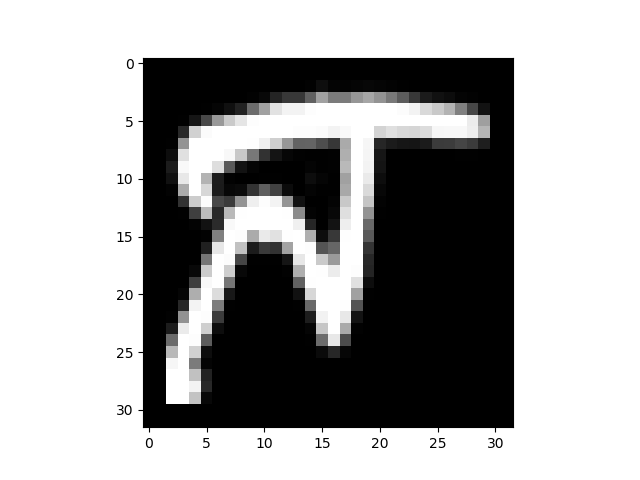
\includegraphics[width=0.3\textwidth]{orig-main.png}
\caption{\label{fig:orig}Original image from the dataset.}
\end{figure}

\begin{figure}[h!]
\centering
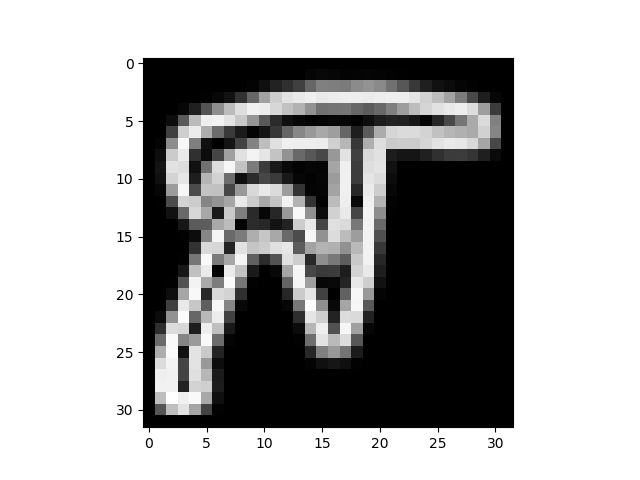
\includegraphics[width=0.3\textwidth]{sobel-main.png}
\caption{\label{fig:sobel}Sobel filter applied to original image.}
\end{figure}

\newpage
\begin{figure} [h!]
\centering
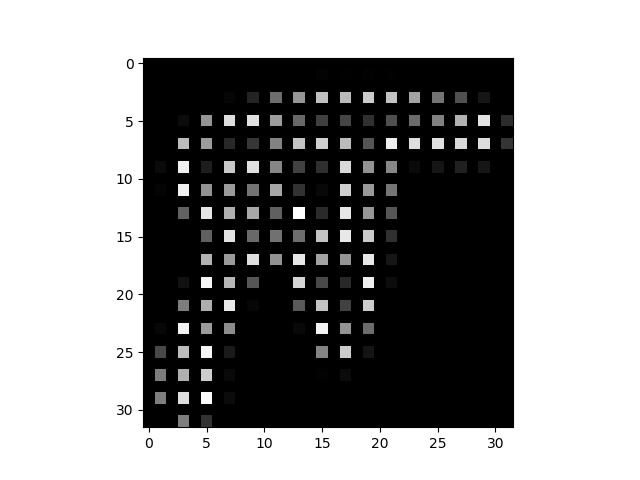
\includegraphics[width=0.3\textwidth]{hog-main.png}
\caption{\label{fig:hog}HOG descriptor applied to original image.}
\end{figure}

\begin{figure} [h!]
\centering
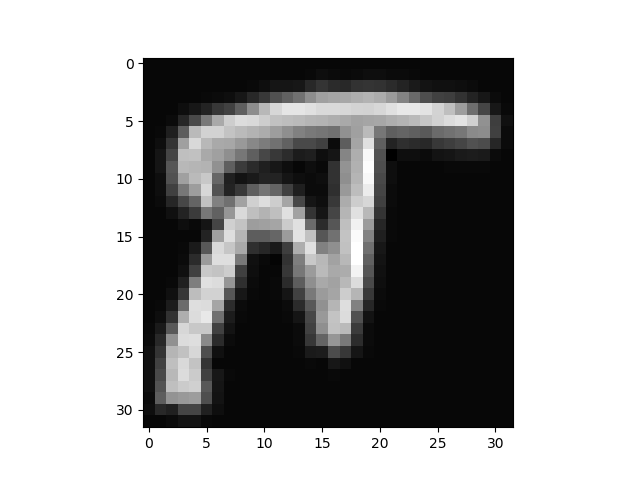
\includegraphics[width=0.3\textwidth]{gabor-main.png}
\caption{\label{fig:gabor}4 Gabor filters applied to original image with max-pooling.}
\end{figure}
\noindent ReLU will be used as the activation function across all the hidden layers because of the problem of saturation in sigmoid (and tanh to some extent) and also because ReLU-based architectures tend to perform better than other activations.
\newline
Softmax activation is used at the output layer, and cross-entropy will be used as the loss function.
\newline
\newline
After trying out the various methods of feature extraction mentioned above, Gabor filters seem to be giving the best validation accuracy. More specifically, for the model: Layers = [500, 300], bs = 100, epochs = 120, lr = 0.2 and 4 Gabor filters with max-pooling, validation accuracy comes out to be 94.5\%, which is the best accuracy that came out from the various architectures tested. So this model was chosen as the final one.
\newline
\newline
This model gave an accuracy of 94.9\% on the public test data.


% \begin{figure}[h!]
% \centering
% 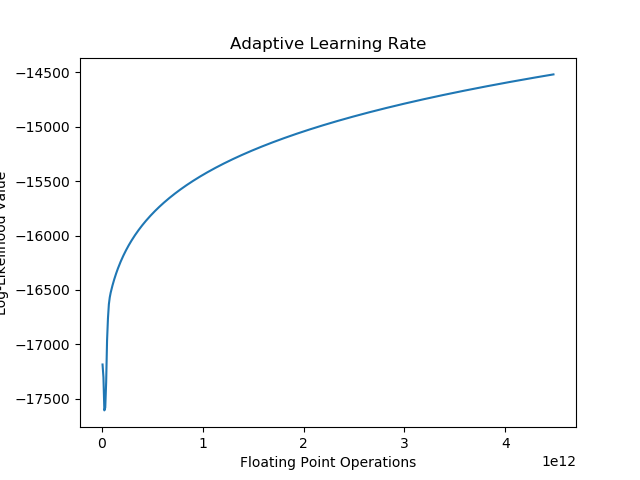
\includegraphics[width=8cm,height=6cm]{adlr_000001_500_65376.png}
% \end{figure}

\end{document}